\begin{note}{Maeva}
   Dans le cours il n'y a pas vraiment d'exemple simple de classe java (il y en a plus dans le cours de la semaine d'après)
   Pour diminuer la charge de travail on pourrait mettre le langage python ou java en exercices avancés
\end{note}

\documentclass[a4paper]{article}
\usepackage{times}
\usepackage[utf8]{inputenc}
\usepackage{selinput}
\usepackage{upquote}
\usepackage[margin=2cm, rmargin=4cm, tmargin=3cm]{geometry}
\usepackage{tcolorbox}
\usepackage{xspace}
\usepackage[french]{babel}
\usepackage{url}
\usepackage{hyperref}
\usepackage{fontawesome5}
\usepackage{marginnote}
\usepackage{ulem}
\usepackage{tcolorbox}
\usepackage{graphicx}
%\usepackage[top=Bcm, bottom=Hcm, outer=Ccm, inner=Acm, heightrounded, marginparwidth=Ecm, marginparsep=Dcm]{geometry}


\newtcolorbox{Example}[1]{colback=white,left=20pt,colframe=slideblue,fonttitle=\bfseries,title=#1}
\newtcolorbox{Solutions}[1]{colback=white,left=20pt,colframe=green,fonttitle=\bfseries,title=#1}
\newtcolorbox{Conseils}[1]{colback=white,left=20pt,colframe=slideblue,fonttitle=\bfseries,title=#1}
\newtcolorbox{Warning}[1]{colback=white,left=20pt,colframe=warning,fonttitle=\bfseries,title=#1}

\setlength\parindent{0pt}

  %Exercice environment
  \newcounter{exercice}
  \newenvironment{Exercice}[1][]
  {
  \par
  \stepcounter{exercice}\textbf{Question \arabic{exercice}:} (\faClock \enskip \textit{#1})
  }
  {\bigskip}
  

% Title
\newcommand{\titre}{\begin{center}
  \section*{Algorithmes et Pensée Computationnelle}
\end{center}}
\newcommand{\cours}[1]
{\begin{center} 
  \textit{#1}\\
\end{center}
  }


\newcommand{\exemple}[1]{\newline~\textbf{Exemple :} #1}
%\newcommand{\attention}[1]{\newline\faExclamationTriangle~\textbf{Attention :} #1}

% Documentation url (escape \# in the TP document)
\newcommand{\documentation}[1]{\faBookOpen~Documentation : \href{#1}{#1}}

% Clef API
\newcommand{\apikey}[1]{\faKey~Clé API : \lstinline{#1}}
\newcommand{\apiendpoint}[1]{\faGlobe~Url de base de l'API \href{#1}{#1}}

%Listing Python style
\usepackage{color}
\definecolor{slideblue}{RGB}{33,131,189}
\definecolor{green}{RGB}{0,190,100}
\definecolor{blue}{RGB}{121,142,213}
\definecolor{grey}{RGB}{120,120,120}
\definecolor{warning}{RGB}{235,186,1}

\usepackage{listings}
\lstdefinelanguage{texte}{
    keywordstyle=\color{black},
    numbers=none,
    frame=none,
    literate=
           {é}{{\'e}}1
           {è}{{\`e}}1
           {ê}{{\^e}}1
           {à}{{\`a}}1
           {â}{{\^a}}1
           {ù}{{\`u}}1
           {ü}{{\"u}}1
           {î}{{\^i}}1
           {ï}{{\"i}}1
           {ë}{{\"e}}1
           {Ç}{{\,C}}1
           {ç}{{\,c}}1,
    columns=fullflexible,keepspaces,
	breaklines=true,
	breakatwhitespace=true,
}
\lstset{
    language=Python,
	basicstyle=\bfseries\footnotesize,
	breaklines=true,
	breakatwhitespace=true,
	commentstyle=\color{grey},
	stringstyle=\color{slideblue},
  keywordstyle=\color{slideblue},
	morekeywords={with, as, True, False, Float, join, None, main, argparse, self, sort, __eq__, __add__, __ne__, __radd__, __del__, __ge__, __gt__, split, os, endswith, is_file, scandir, @classmethod},
	deletekeywords={id},
	showspaces=false,
	showstringspaces=false,
	columns=fullflexible,keepspaces,
	literate=
           {é}{{\'e}}1
           {è}{{\`e}}1
           {ê}{{\^e}}1
           {à}{{\`a}}1
           {â}{{\^a}}1
           {ù}{{\`u}}1
           {ü}{{\"u}}1
           {î}{{\^i}}1
           {ï}{{\"i}}1
           {ë}{{\"e}}1
           {Ç}{{\,C}}1
           {ç}{{\,c}}1,
    numbers=left,
}

\newtcbox{\mybox}{nobeforeafter,colframe=white,colback=slideblue,boxrule=0.5pt,arc=1.5pt, boxsep=0pt,left=2pt,right=2pt,top=2pt,bottom=2pt,tcbox raise base}
\newcommand{\projet}{\mybox{\textcolor{white}{\small projet}}\xspace}
\newcommand{\optionnel}{\mybox{\textcolor{white}{\small Optionnel}}\xspace}
\newcommand{\advanced}{\mybox{\textcolor{white}{\small Pour aller plus loin}}\xspace}
\newcommand{\auto}{\mybox{\textcolor{white}{\small Auto-évaluation}}\xspace}


\usepackage{environ}
\newif\ifShowSolution
\NewEnviron{solution}{
  \ifShowSolution
	\begin{Solutions}{\faTerminal \enskip Solution}
		\BODY
	\end{Solutions}
  \fi}


  \usepackage{environ}
  \newif\ifShowConseil
  \NewEnviron{conseil}{
    \ifShowConseil
    \begin{Conseils}{\faLightbulb \quad Conseil}
      \BODY
    \end{Conseils}

    \fi}

    \usepackage{environ}
  \newif\ifShowWarning
  \NewEnviron{attention}{
    \ifShowWarning
    \begin{Warning}{\faExclamationTriangle \quad Attention}
      \BODY
    \end{Warning}

    \fi}
  

%\newcommand{\Conseil}[1]{\ifShowIndice\ \newline\faLightbulb[regular]~#1\fi}


\usepackage{array}
\newcolumntype{C}[1]{>{\centering\let\newline\\\arraybackslash\hspace{0pt}}m{#1}}

\begin{document}
% Change the following values to true to show the solutions or/and the hints
\ShowSolutiontrue
\ShowConseiltrue
\titre
\cours{Programmation orientée objet}

Le but de cette séance est de se familiariser avec un paradigme de programmation couramment utilisé: la Programmation Orientée Objet (POO). Ce paradigme consiste en la définition et en l'intéraction avec des briques logicielles appelées \lstinline{Objets}. Dans les exercices suivants, nous manipulerons des objets, aborderons les notions de classe, méthodes, attributs et encapsulation. Au terme de cette séance, vous serez en mesure d'écrire des programmes mieux structurés.
Afin d'atteindre ces objectifs, nous utiliserons principalement le langage \lstinline{Java} qui offre une panoplie d'outils pour mieux comprendre ce paradigme de programmation.
\\
%TODO: Rajouter un lien vers les vidéos

Le code présenté dans les énoncés se trouve sur Moodle, dans le dossier \lstinline{Ressources}.

\section{Création de votre première classe en Java}

Le but de cette première partie est de créer votre propre classe en Java. Cette classe sera une classe nommée \lstinline{Dog()} représentant un chien. Elle aura plusieurs attributs et méthodes que vous implémenterez au fur et à mesure.

\begin{Exercice}[10 minutes] Création de classe et encapsulation\\
    Commencez par créer une nouvelle classe \lstinline{Java} dans votre projet, et initialisez les attributs suivants :
    \begin{enumerate}
    \item Un attribut \lstinline{public} String nommé \lstinline{name}
    \item Un attribut \lstinline{private} List nommé \lstinline{tricks}
    \item Un attribut \lstinline{private} String nommé \lstinline{race}
    \item Un attribut \lstinline{private} int nommé \lstinline{age}
    \item Un attribut \lstinline{private} int nommé \lstinline{mood} initialisé à 5 (correspondant à l'humeur du chien)
    \item Un attribut de classe (\lstinline{static}) \lstinline{private} int nommé \lstinline{nb_chiens}
   	\end{enumerate}
   	
   	Ensuite, créez une méthode publique du même nom que la classe (\lstinline{Dog}). Cette méthode est appelée le \lstinline{constructeur}, elle va servir à initialiser les différentes instances de notre classe. Un \lstinline{constructeur} en \lstinline{Java} aura le même nom que la classe, et un \lstinline{constructeur} en \lstinline{python} sera la méthode \lstinline{__init__}. Cette méthode prendra en argument les éléments suivants et initialisera les attributs de notre instance :
   	\begin{enumerate}
    \item Une chaîne de caractère \lstinline{name}
    \item Une liste \lstinline{tricks}
    \item Une chaîne de caractère \lstinline{race}
    \item Un entier \lstinline{age}
   	\end{enumerate}
   	
   	Pour finir, cette méthode doit incrémenter l'attribut de classe \lstinline{nb_chiens} qui va garder en mémoire le nombre d'instances crées.
   	
\begin{conseil}
   N'oubliez pas de préciser si vos attributs sont \lstinline{public} ou \lstinline{private}.
   
   Le mot \lstinline{static} correspond à un élément de classe (attribut ou méthode), cet élément pourra ensuite être appelé via la classe directement.
   
   Pour attribuer des valeurs à vos attributs d'instance, utilisez le mot-clé \lstinline{this.attribut}.
   
   Pour accéder aux attributs de classe, utilisez \lstinline{nom_classe.nom_attribut}
\end{conseil}
    
\begin{solution}
	\lstinputlisting{ressources/Question1.java}
\end{solution}
\end{Exercice}

\begin{Exercice}[10 minutes] Getters et setters\\
    Il faut maintenant créer des méthodes nommées \lstinline{setter} et \lstinline{getter} pour les attributs privés. Ce sont ces méthodes qui vous permettront d'interagir avec les attributs \lstinline{private} des instances de la classe. Pour les attributs publics, il vous suffit d'utiliser \lstinline{nom_instance.attribut} pour l'obtenir. \\
    
    Les méthodes \lstinline{getter} d'accéder à la valeur d'un attribut. Les \lstinline{setter} permettent de modifier la valeur de l'attribut. Les \lstinline{setter} sont souvent utilisés pour modifier la valeur d'attributs privés. \\
    
    Créez les méthodes suivantes :
    \begin{itemize}
    \item \lstinline{getTricks()}
    \item \lstinline{getRace()}
    \item \lstinline{getAge()}
    \item \lstinline{getMood()}
    \item \lstinline{setTricks()}
    \item \lstinline{setRace()}
    \item \lstinline{setAge()}
    \item \lstinline{setMood()}
    \end{itemize}
    
    Créez également une méthode de classe permettant de retourner le nombre de \lstinline{Dog} instanciés (une méthode \lstinline{getter}).
   	
\begin{conseil}
    Intellij vous permet de générer automatiquement certaines méthodes telles que les getters et setters. Vous pouvez consulter le lien suivant pour plus d'informations: \url{https://www.jetbrains.com/help/idea/generating-code.html\#generate-delegation-methods}.
    \\
    Toutefois, pour cet exercice, nous vous encourageons à le faire manuellement.
\end{conseil}
    
\begin{solution}
	\lstinputlisting{ressources/Question2.java}
\end{solution}
\end{Exercice}

\begin{Exercice}[5 minutes] Manipulation d'attributs - Listes\\
    Créez une méthode \lstinline{public} nommée \lstinline{add_trick(String trick)} qui prend en entrée une chaîne de caractère et l'ajoute à la liste \lstinline{tricks}. \\
   	
\begin{conseil}
   La liste \lstinline{tricks} est une liste comme les autres. Si vous voulez la modifier, vous aurez besoin de passer par une \lstinline{LinkedList} temporaire.
\end{conseil}
    
\begin{solution}
	\lstinputlisting{ressources/Question3.java}
\end{solution}
\end{Exercice}

\begin{Exercice}[5 minutes] Manipulation d'attributs - setter\\
    Créez deux méthodes qui vont avoir un impact sur l'attribut \lstinline{mood} du \lstinline{Dog}. La méthode \lstinline{leash()} décrémentera mood de 1 et \lstinline{eat()} l'incrémentera de 3. \\

\begin{solution}
	\lstinputlisting{ressources/Question4.java}
\end{solution}
\end{Exercice}

\begin{Exercice}[5 minutes] Manipulation d'attributs d'une autre instance\\
    Créez une méthode nommée \lstinline{get_oldest(Dog other)} qui prend comme argument un élément de type \lstinline{Dog}, puis retourne le nom et l'age du \lstinline{Dog} le plus agé sous le format suivant : "\lstinline{nom_chien} est le chien le plus agé avec \lstinline{age_chien} ans". \\
   	
\begin{conseil}
   L'élément \lstinline{Dog} que vous passez en argument est un objet de type \lstinline{Dog}, vous pouvez donc lui appliquer les méthodes que vous avez créé tout à l'heure.
   Faites attention à la façon d'accéder aux différents attributs de votre deuxième chien (\lstinline{public} vs \lstinline{private}).
\end{conseil}
    
\begin{solution}
	\lstinputlisting{ressources/Question5.java}
\end{solution}
\end{Exercice}

\begin{Exercice}[5 minutes] Redéfinition de méthodes\\
    Créez une méthode \lstinline{toString()} qui retourne une chaîne de caractères contenant toutes les informations d'une instance de \lstinline{Dog}. Ainsi, dans votre \lstinline{main}, en faisant \lstinline{System.out.println(...)} sur une instance de \lstinline{Dog}, vous obtiendrez une texte sous le format suivant: 
    \lstinline{nom_chien} a \lstinline{age_chien} ans, est un \lstinline{race_chien} et a une humeur de \lstinline{mood_chien}. Il sait faire les tours suivants : \lstinline{tricks_chien}.

    \begin{Example}{\faLightbulb \quad Informations utiles}
        La méthode \lstinline{toString()} hérite de la super classe Object. La notion d'héritage sera présentée la semaine prochaine. Retenez juste qu'il est possible de choisir ce que vaudra le texte descriptif de nos objets de type \lstinline{Dog}. Il est également possible de redéfinir d'autres méthodes comme par exemple l'addition ou la soustraction, ce qui permettrait de choisir comment 2 objets de type \lstinline{Dog} seraient additionnés ou soustraits. \\
    \end{Example}

    \begin{solution}
        \lstinputlisting{ressources/Question6.java}
    \end{solution}
\end{Exercice}

Pour contrôler que vos méthodes et attributs ont été implémentés correctement, vous pouvez essayer le code suivant dans votre classe Main :

	\lstinputlisting{ressources/question6_main.java}
	
Vous devriez obtenir ce résultat :
    \lstinputlisting{ressources/mainsolution.java}

\newpage
\section{Interaction entre plusieurs instances d'une même classe}
Dans cette section, nous allons simuler un jeu de combat entre deux protagonistes représentant des instances d'une classe \lstinline{Fighter} que nous allons créer.
Chaque \lstinline{Fighter} aura des attributs qui le définissent. Ces attributs sont:
\begin{itemize}
    \item \lstinline{nom:}\textit{(String)} chaque combattant sera identifié par un nom unique.
    \item \lstinline{health:}\textit{(int)} représentant le nombre de points de vie d'un combattant. Il contient des valeurs comprises entre 0 et 10. À l'instanciation de l'objet, le combattant a 10 points de vie par défaut.
    \item \lstinline{attaque:}\textit{(int)} représentant une valeur qui sera utilisée pour calculer le nombre de points de dégâts infligés à l'adversaire.
    \item \lstinline{défense:}\textit{(int)} représentant une valeur qui sera utilisée pour calculer le nombre de points de dégâts reçus.
\end{itemize}

2 attributs de classe seront également utilisés :
\begin{itemize}
\item \lstinline{instances :} Liste comprenant les combattants qui ont été instanciés et qui sont toujours en vie.
\item \lstinline{attack_modifier :} Dictionnaire comportant 3 types d'attaques, chacune modifiant les dégâts qui vont être infligés. Les trois types d'attaques sont \lstinline{poing, pied et tête} modifiant respectivement l'attaque par 1, 2, 3.
\end{itemize}

Le but de cette partie est d'étudier les interactions entre deux instances d'une même classe. Cette classe se présentera sous la forme d'un \lstinline{Fighter}. Chaque instance de cette classe pourra attaquer les autres instances.

Vous devrez compléter les 4 méthodes suivantes :
\begin{enumerate}
\item \lstinline{isAlive()}
\item \lstinline{checkDead()}
\item \lstinline{checkHealth()}
\item \lstinline{attack(String type, Fighter other)}
\end{enumerate}




Voici le squelette du code (à télécharger sur Moodle) : \\

\lstinputlisting{ressources/fighter.java}

\begin{Exercice}[5 minutes] isAlive()\\
    Définir une méthode \lstinline{isAlive()} qui retournera \lstinline{true} si l'instance a plus que 0 points de vie et \lstinline{false} si l'instance en a moins.

\begin{solution}
	\lstinputlisting{ressources/isalive.java}
\end{solution}
\end{Exercice}


\begin{Exercice}[10 minutes] checkDead()\\
    Définir une méthode \lstinline{checkDead()} qui consiste à parcourir la liste des instances, et à contrôler que chacune d'elle est encore en vie. Si ce n'est pas le cas, l'instance en question est supprimée de la liste des instances et le message ``\lstinline{nom_instance} est mort'' sera affiché.
    
\begin{conseil}
Prenez le problème dans l'autre sens, créez une liste temporaire, si l'instance est vivante ajoutez la à cette nouvelle liste, et pour finir, mettez à jour votre liste d'instances à l'aide de votre liste temporaire.
\end{conseil}

\begin{solution}
	\lstinputlisting{ressources/checkdead.java}
\end{solution}
\end{Exercice}

\begin{Exercice}[5 minutes] checkHealth()\\
    Définir une méthode \lstinline{checkHealth()} qui parcourt la liste des instances et imprime le nombre de points de vie qui reste au combattant sous le format ``\lstinline{nom_instance} a encore \lstinline{health_instance} points de vie". 

\begin{solution}
	\lstinputlisting{ressources/checkhealth.java}
\end{solution}
\end{Exercice}

\begin{Exercice}[10 minutes] attack(String type Fighter other)\\
    Définir une méthode \lstinline{attack(String type, Fighter other)} qui consiste à retirer des points de vie au combattant \lstinline{other} en fonction de l'attaque de l'instance appelée, du type d'attaque sélectionné et de la défense de \lstinline{other}. \\
    
    Commencez par contrôler si \lstinline{other} est encore en vie, si ce n'est pas le cas, indiquez qu'il est déjà mort : ``\lstinline{other_name} est déjà mort". \\
    
     Si \lstinline{other} est encore en vie, retirez des points de vie à \lstinline{other}. Le nombre de points de vie devant être retiré se calcule en utilisant la formule suivante : \lstinline{attack_modifier(type)} * \lstinline{attack_instance} - \lstinline{defense_other}. Appelez ensuite les fonctions \lstinline{checkDead()} et \lstinline{checkHealth()} afin d'avoir un aperçu des combattants restants et de leur santé.
    


\begin{solution}
	\lstinputlisting{ressources/attack.java}
\end{solution}
\end{Exercice}


Pour terminer, vous pouvez exécuter le code ci-dessous (disponible dans le dossier Ressources sur Moodle) pour vérifier que votre programme fonctionne correctement : \\

\lstinputlisting{ressources/main2.java}

Vous devriez obtenir ce résultat : \\

\lstinputlisting{ressources/main2solution.java}

\newpage

\section{Manipulation de graphes en POO (Java)}

%\subsection{Introduction}
% TODO: Cette sous-section devrait être convertie en introduction. Les questions sont intéressantes. Toutefois, elles perdent de leur utilité si les étudiants n'ont pas accès aux réponses de façon immédiate. Il serait préférable de les reformuler et de les utiliser comme rappel avant de commencer à faire les exercices suivants.


%Ici, on cherche à pousser votre réflexion sur le processus de conception de classes pour implémenter un concept existant en dehors de la programmation.
%Pour cela, il faut se placer du point de vue de l'utilisateur pour savoir ce dont il aurait besoin. 
%Il faut aussi savoir de quoi est constitué le concept que l'on cherche à implémenter. C'est-à-dire, pour utiliser une analogie, les différentes briques qui sont utilisées pour construire le mur qui est votre objet final.

Cette partie constitue un rappel sur la notion de graphe orienté. Avant de traiter les exercices de la partie 2, veuillez répondre aux questions suivantes:
    \begin{enumerate}
        \item Quels sont les composantes d'un \lstinline{graphe orienté} ?
        \item Combien de classes sont nécessaires pour représenter un graphe orienté ainsi que toutes ses composantes?
        \item Sachant que vous avez une classe qui représente les \lstinline{arêtes} et que les \lstinline{sommets} sont représentés par des chaînes de caractères. Quels pourraient être les attributs de la classe \lstinline{graph}.
    \end{enumerate}

Maintenant que vous avez une idée des attributs de la classe \lstinline{graph} à définir, déterminer quelles méthodes sont nécessaires au fonctionnement de cet objet. Pour ce faire, vous pouvez répondre aux questions suivantes:
    \begin{enumerate}
    \item Est-ce que l'utilisateur aura besoin de modifier l'objet une fois celui-ci initialisé ?
    \item Est-ce que l'utilisateur aura besoin de vérifier l'état de l'objet (existence d'attributs, vérification de valeurs...) ou de certaines parties de l'objet ?
    \end{enumerate}

\begin{conseil}
   % Un conseil
   \begin{enumerate}
   \item Revenir sur le cours de la semaine 7 sur Moodle.
   \end{enumerate}
\end{conseil}
    
Voici les réponses aux questions posées ci-dessus. 

\textbf{Certaines questions peuvent avoir plus d'une réponse étant donné qu'il existe plusieurs manières de représenter un graphe en programmation. }
    %\lstinputlisting{solutions/fichier.java}
    \begin{enumerate}
    \item \begin{enumerate}
          \item Les \lstinline{sommets}.
          \item Les \lstinline{arêtes}.
          \item Le \lstinline{poids} de chaque arête.
          \end{enumerate}
    \item Il faut 2 classes ( ou 3 si on cherche à avoir plus d'informations dans les sommets):
        \begin{enumerate}
        \item Une classe \lstinline{Edge} qui va représenter les arêtes.
        \item Une classe \lstinline{Graph}.
        \end{enumerate}
    \item La classe \lstinline{Graph} va avoir 2 attributs: un ensemble contenant les \lstinline{sommets} et un autre ensemble contenant les \lstinline{arêtes} de celui-ci.
    
%    \item Les réponses à cette partie sont courtes mais assez essentielles pour savoir quelles méthodes coder:
 %       \begin{enumerate}
       % \item Oui, l'utilisateur voudra sûrement rajouter des \lstinline{arêtes}, des \lstinline{sommets} ou potentiellement changer le poids d'une \lstinline{arête}. Il faut donc lui laisser cette possibilité
       % \item Les graphs sont souvent accompagnés par des algorithmes de recherche, par exemple l'algorithme de Kruskal pour les \lstinline{weighted graphs}. Il est donc utile de pouvoir identifier si un \lstinline{sommet} ou une \lstinline{arête} sont des composants de l'instance.
       % \item Certaines méthodes pourraient avoir un code très long si on ne ségmentarise pas leur contenu. Cela peut entraver la relecture de votre code par vous ou par un tiers. 
        
       % De plus dans un cadre d'optimisation, il faut éviter un maximum la redondance du code. Il est donc de bonne pratique de définir des méthodes qui vont éviter cela dans une classe.
  %      \end{enumerate}
    \end{enumerate}

%\subsection{Partie 2}
% TODO: Edge doit être mis au singulier pour éviter qu'ils ne confondent l'objet à son instance.

Le code de la classe \lstinline{Edge} est fourni dans le dossier ressources sur Moodle.
Utiliser le fichier \lstinline{Main.java} dans le dossier \lstinline{Ressources} sur Moodle pour effectuer des tests. Une fois exécuté, il devrait afficher:\\

    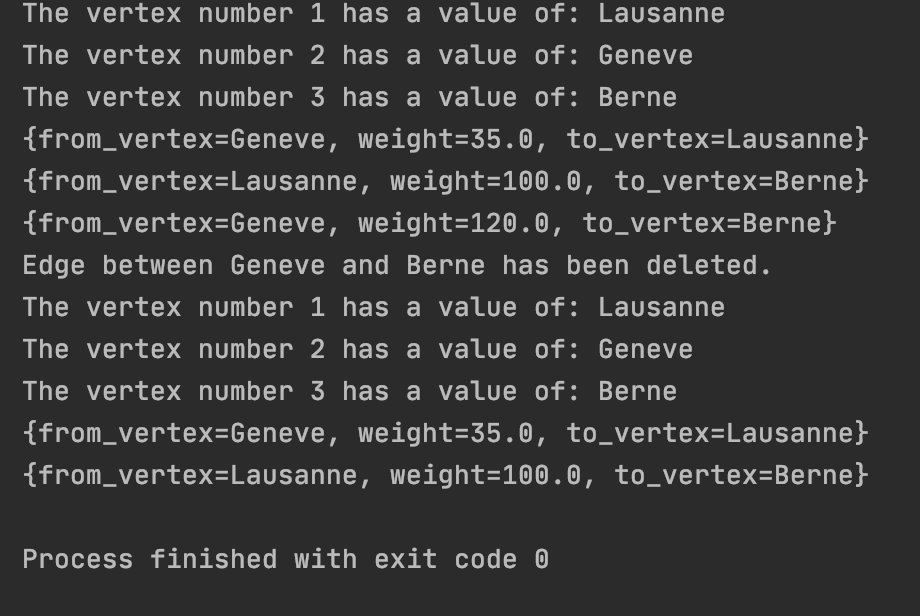
\includegraphics[height=8cm]{ressources/sortie_juste.PNG}

\newpage

\begin{note}{Maeva}
    Ceci devrait être un exercice avancé
\end{note}
\begin{Exercice}[20 minutes]\\

Voici une partie de la classe \lstinline{graph} codée. Implémentez les méthodes \lstinline{update_weight()}, \lstinline{new_edge} et \lstinline{edge_exist}.

         \lstinputlisting{ressources/graph_empty.java}
    \begin{enumerate}
        \item La méthode \lstinline{update_weight()} doit prendre en paramètres: le \lstinline{sommet} d'origine, le \lstinline{sommet} d'arrivée ainsi que le poids d'une \lstinline{arête}. Si cette \lstinline{arête} existe alors elle change son poids. Sinon, elle imprimera une phrase indiquant que l'\lstinline{arête} n'existe pas.
        \item La méthode \lstinline{edge_exist()} prendra en paramètre le \lstinline{sommet} d'origine et le \lstinline{sommet} d'arrivée. Si cette \lstinline{arête} est dans le \lstinline{graph} alors la méthode renvoie son poids, sinon, elle renvoie 0.
        \item La méthode \lstinline{new_edge} doit créer une instance de \lstinline{Edge} et l'ajouter à l'ensemble edges si la connexion n'existe pas déjà. Si elle existe avec un autre poids mettre à jour le poids. Si elle existe de façon identique alors retournez la dans la console avec print. Enfin, si on est dans aucun des deux cas précédents utiliser la méthode \lstinline{generate_edge} qui vous est donnée pour créer et ajouter cette arête au \lstinline{graph}. La méthode \lstinline{new_edge} aura pour paramètres: le \lstinline{sommet} d'origine, le \lstinline{sommet} d'arrivée, le poids.
    \end{enumerate}

    \begin{conseil}
    \begin{enumerate}
    \item Utiliser une boucle \lstinline{for} pour parcourir toutes les \lstinline{arêtes} dans le \lstinline{graph}. Faire un test sur les attributs de \lstinline{Edge} pour changer le poids.
    \item Il faut tester pour chaque \lstinline{arête} ( itération) si elle  est égale à celle donnée en paramètres.
    \item Il faut utiliser les méthodes \lstinline{edge_exist()}, \lstinline{update_edge()} et \lstinline{generate_edge()} pour écrire cette méthode. Il y a 4 tests à effectuer: 
        \begin{enumerate}
        \item Si \lstinline{l'arête} existe.
        \item Si \lstinline{l'arête} existante a le même poids que celle indiquée en paramètre de la méthode.
        \item Si \lstinline{l'arête} existante n'a pas le même poids que celle indiquée en paramètre de la méthode.
        \item Utilisez le résultat de \lstinline{edge_exist} pour simplifier ces tests.
        \end{enumerate}
    \end{enumerate}
    \end{conseil}
    \begin{solution}
    \textbf{Java :}
         \lstinputlisting{ressources/Edge.java}
    \end{solution}
    \begin{solution}
    \textbf{Java :}
         \lstinputlisting{ressources/graph.java}
    \end{solution}
    % TODO: Découper les fichiers de solutions pour qu'ils tiennent sur une page. Les renommer graph_1.java, graph_2,java par exemple et les mettre dans un dossier "Display" ou "Affichage". Mettre le fichier complet dans le dossier solution.
    \begin{solution}
    \textbf{Java :}
         \lstinputlisting{ressources/graph2.java}
    \end{solution}

\end{Exercice}

\newpage

\section{Notions de POO en Python}
Dans cette section, nous créerons pas-à-pas une classe \lstinline{Point} contenant des attributs et des méthodes utiles.
Dans votre IDE, créez un nouveau projet Python (Fichier \> Nouveau \> Projet). Dans un dossier de votre choix, créez un fichier \lstinline{question12.py}.

\begin{Exercice}[15 minutes] Classe Point
    \begin{itemize}
        \item Créez une classe \lstinline{Point} et un constructeur par défaut contenant deux paramètres (x et y).
        \begin{conseil}
            Pour rappel, un constructeur est une fonction \lstinline{__init()__} que vous redéfinirez dans votre classe.
        \end{conseil}
        \item Définissez deux attributs privés pour votre classe \lstinline{Point}. Ces attributs seront les coordonnées x et y de vos points. Par défaut, assignez leur les valeurs données dans le constructeur.
        \begin{conseil}
            À l'intérieur d'une classe, utilisez le mot-clé \lstinline{self} pour accéder aux méthodes et attributs de l'instance que vous manipulez.

            En Python, pour spécifier qu'un attribut est privé, rajouter un double underscore au nom de l'attribut (Exemple: \lstinline{__score=0})
        \end{conseil}
        \item Définir des getters et setters.
        \begin{conseil}
            En Python, le mot-clé \lstinline{self} est l'équivalent de \lstinline{this} utilisé en Java.
        \end{conseil}
        \item Définissez une méthode \lstinline{distance} qui prend en entrée l'instance du Point (\lstinline{self}) et une autre point \lstinline{p2}. Cette méthode \lstinline{distance} retournera la distance euclidienne entre le point \lstinline{self} et \lstinline{p2}. 
        \begin{conseil}
            Pour rappel, la distance euclidienne entre deux points est définie par la formule $\sqrt{(x_1 - x_2)^2 + (y_1 - y_2)^2}$.

            Utilisez la fonction \lstinline{sqrt()} de la librairie \lstinline{math} pour calculer la racine carrée. Pensez à importer la libraire \lstinline{math}
        \end{conseil}
        \item Définissez une méthode \lstinline{milieu} qui prendra en entrée \lstinline{self} et \lstinline{p2} et qui retournera un objet \lstinline{Point} situé entre \lstinline{self} et \lstinline{p2}.
        \begin{conseil}
            Pour trouver les coordonnées d'un point M($x_M$, $y_M$) situé au milieu du segment défini par des points A($x_A$, $y_A$) et B($x_B, y_B$),
            utilisez les formules suivantes:
            $x_M = \frac{x_1 + x_2}{2}$ et $y_M = \frac{y_1 + y_2}{2}$
        \end{conseil}

        \item Redéfinissez une méthode \lstinline{__str__()} dans la classe \lstinline{Point} qui retournera une chaîne de caractères contenant les coordonnées $(x,y)$ d'un point. Ainsi, lorsqu'on fera un \lstinline{print} d'une instance de la classe \lstinline{Point}, le message qui s'affichera sera le suivant:
        \textit{Les coordonnées du Point sont: x = "remplacez par la valeur de x" et y = "remplacez par la valeur de y"}
    \end{itemize}

\end{Exercice}

\begin{solution}
    \lstinputlisting{solutions/question12_solution.py}
\end{solution}

\end{document}
